\documentclass[12pt,a4paper]{article}

%%%%%%%%%%%%%%%%%%%%%%%%%%%%%%%%%%%%%%%%%%%%%%%%%%%%%%%%%%%%%%%%%%%%%%%%%%%%
% 1. FONTS: Times-style text and math font.
%    Alternatives (swap this block):
%      Libertine:  \usepackage{libertine} + \usepackage[libertine]{newtxmath}
%      XCharter:   \usepackage{xcharter}
%%%%%%%%%%%%%%%%%%%%%%%%%%%%%%%%%%%%%%%%%%%%%%%%%%%%%%%%%%%%%%%%%%%%%%%%%%%%
\usepackage{newtxtext}

%%%%%%%%%%%%%%%%%%%%%%%%%%%%%%%%%%%%%%%%%%%%%%%%%%%%%%%%%%%%%%%%%%%%%%%%%%%%
% 2. MICROTYPOGRAPHY: subtle spacing tweaks for cleaner justified text.
%%%%%%%%%%%%%%%%%%%%%%%%%%%%%%%%%%%%%%%%%%%%%%%%%%%%%%%%%%%%%%%%%%%%%%%%%%%%
\usepackage{microtype}

%%%%%%%%%%%%%%%%%%%%%%%%%%%%%%%%%%%%%%%%%%%%%%%%%%%%%%%%%%%%%%%%%%%%%%%%%%%%
% 3. LANGUAGE & ENCODING: special characters + hyphenation rules.
%    Swap "english" for your language if needed, e.g.:
%      \usepackage[ngerman]{babel}   % German
%      \usepackage[french]{babel}    % French
%    This automatically updates hyphenation patterns and auto-generated
%    text like "Figure"/"Abbildung" without touching anything else here.
%%%%%%%%%%%%%%%%%%%%%%%%%%%%%%%%%%%%%%%%%%%%%%%%%%%%%%%%%%%%%%%%%%%%%%%%%%%%
\usepackage[utf8]{inputenc}
\usepackage[T1]{fontenc}
\usepackage{lmodern}
\usepackage[english]{babel}
\hyphenpenalty=1000
\exhyphenpenalty=50
\tolerance=1000

%%%%%%%%%%%%%%%%%%%%%%%%%%%%%%%%%%%%%%%%%%%%%%%%%%%%%%%%%%%%%%%%%%%%%%%%%%%%
% 4. MATH: equations, symbols, theorem environments, bold vectors.
%%%%%%%%%%%%%%%%%%%%%%%%%%%%%%%%%%%%%%%%%%%%%%%%%%%%%%%%%%%%%%%%%%%%%%%%%%%%
\usepackage{amsmath}
\usepackage{amssymb}
\usepackage{amsthm}
\usepackage{mathtools}
\usepackage{bm}
\usepackage{newtxmath} % load after amsmath; swap if using an alt font (see above)
\let\openbox\relax     % avoids a naming clash between amsthm and another package

%%%%%%%%%%%%%%%%%%%%%%%%%%%%%%%%%%%%%%%%%%%%%%%%%%%%%%%%%%%%%%%%%%%%%%%%%%%%
% 5. GRAPHICS, FIGURES & TABLES
%
%    TIP: Building tables by hand is tedious and error-prone, especially
%    regression output tables (coefficients, standard errors, significance
%    stars, footnotes). Recommended workflow instead:
%      1. Run your regression in R (or Python/Stata) and export the raw
%         output, or just take a screenshot of the R console/table.
%      2. Paste the R output or screenshot into an AI assistant and ask it
%         to generate a LaTeX table using booktabs (\toprule, \midrule,
%         \bottomrule) that matches your regression results.
%      3. Compile the generated code as-is, then manually tweak only small
%         details afterward: column widths, number formatting, footnote
%         text for significance levels (e.g. * p<0.10, ** p<0.05), or
%         table width via adjustbox if it overflows the page margin.
%    This is far faster than manually transcribing coefficients and gets
%    you a clean, publication-style table (similar to R's stargazer or
%    modelsummary output) without writing raw tabular code by hand.
%%%%%%%%%%%%%%%%%%%%%%%%%%%%%%%%%%%%%%%%%%%%%%%%%%%%%%%%%%%%%%%%%%%%%%%%%%%%
\usepackage{graphicx}
\usepackage{float}
\usepackage{caption}
\usepackage{subcaption}
\usepackage{booktabs}
\usepackage{array}
\usepackage{multirow}
\usepackage{rotating}
\usepackage{lscape}
\usepackage{pdflscape}
\usepackage{adjustbox}
\usepackage{tcolorbox}

%%%%%%%%%%%%%%%%%%%%%%%%%%%%%%%%%%%%%%%%%%%%%%%%%%%%%%%%%%%%%%%%%%%%%%%%%%%%
% 6. UNITS (OPTIONAL): only needed for physical units or numeric tables
%    that require consistent decimal alignment, e.g. "3.14 kg".
%    Comment out if you don't work with measurements/units.
%%%%%%%%%%%%%%%%%%%%%%%%%%%%%%%%%%%%%%%%%%%%%%%%%%%%%%%%%%%%%%%%%%%%%%%%%%%%
% \usepackage{siunitx}
% \sisetup{detect-all}

%%%%%%%%%%%%%%%%%%%%%%%%%%%%%%%%%%%%%%%%%%%%%%%%%%%%%%%%%%%%%%%%%%%%%%%%%%%%
% 7. TEXT DECORATION & LISTS
%%%%%%%%%%%%%%%%%%%%%%%%%%%%%%%%%%%%%%%%%%%%%%%%%%%%%%%%%%%%%%%%%%%%%%%%%%%%
\usepackage{enumitem}
\usepackage[normalem]{ulem} % enables \sout{} strikethrough

%%%%%%%%%%%%%%%%%%%%%%%%%%%%%%%%%%%%%%%%%%%%%%%%%%%%%%%%%%%%%%%%%%%%%%%%%%%%
% 8. DIAGRAMS (OPTIONAL): TikZ for custom diagrams/flowcharts drawn in code.
%
%    TIP: Writing TikZ by hand is painful, especially node positioning and
%    arrows. Recommended workflow instead:
%      1. Describe the diagram to an AI assistant (e.g. "causal diagram
%         showing X affects Y through mediator Z, with labeled arrows")
%         and ask it to generate the TikZ code.
%      2. Compile the generated code as-is to see the rough layout.
%      3. Manually tweak only the fine details afterward: node coordinates
%         (via the "positioning" library, e.g. right=of, below=of),
%         arrow styles, and spacing values, since these are the parts
%         AI often gets slightly off but are easy to nudge by eye.
%    TikZ is very flexible this way: flowcharts, causal mechanisms,
%    timelines, or statistical illustrations all render as crisp vector
%    graphics that scale perfectly in the final PDF, unlike a screenshot.
%    Uncomment only if you actually plan to draw diagrams in LaTeX.
%%%%%%%%%%%%%%%%%%%%%%%%%%%%%%%%%%%%%%%%%%%%%%%%%%%%%%%%%%%%%%%%%%%%%%%%%%%%
\usepackage{tikz}
\usetikzlibrary{arrows.meta,positioning,fit,calc,decorations.pathreplacing}

%%%%%%%%%%%%%%%%%%%%%%%%%%%%%%%%%%%%%%%%%%%%%%%%%%%%%%%%%%%%%%%%%%%%%%%%%%%%
% 9. COLORS: custom color definitions used in tables/highlights.
%%%%%%%%%%%%%%%%%%%%%%%%%%%%%%%%%%%%%%%%%%%%%%%%%%%%%%%%%%%%%%%%%%%%%%%%%%%%
\usepackage{xcolor}
\usepackage{colortbl}
\definecolor{regblue}{RGB}{220, 230, 242}
\definecolor{headerblue}{RGB}{169, 196, 223}
\definecolor{emptycell}{RGB}{245, 245, 245}

%%%%%%%%%%%%%%%%%%%%%%%%%%%%%%%%%%%%%%%%%%%%%%%%%%%%%%%%%%%%%%%%%%%%%%%%%%%%
% 10. BIBLIOGRAPHY: author-year citations (natbib/plainnat = Harvard style,
%     common in economics).
%       See folder Front Matter and then document "bibliography_setup.tex" for      explaination how it works.
%       If you want to edit, edit in "bibliography_setup.tex".
%%%%%%%%%%%%%%%%%%%%%%%%%%%%%%%%%%%%%%%%%%%%%%%%%%%%%%%%%%%%%%%%%%%%%%%%%%%%
%%%%%%%%%%%%%%%%%%%%%%%%%%%%%%%%%%%%%%%%%%%%%%%%%%%%%%%%%%%%%%%%%%%%%%%%%%%%
% BIBLIOGRAPHY: author-year citations (natbib/plainnat = Harvard style,
%     common in economics).
%
%     HOW CITATIONS WORK (mechanism explained):
%     - All sources live in a separate plain-text file, e.g. references.bib,
%       NOT in this .tex file. Each entry has a unique key (e.g. smith2020)
%       plus fields like author, title, year, journal.
%     - \bibliography{references} at the END of your document (without the
%       .bib extension) tells LaTeX which file to pull from.
%     - \bibliographystyle{plainnat} below controls the FORMAT of both the
%       in-text citations and the final reference list. You never type the
%       full reference yourself; it's auto-generated from the .bib fields.
%     - \citep{smith2020}  ->  "(Smith, 2020)"   use when the name is NOT
%       part of your sentence grammar.
%     - \citet{smith2020}  ->  "Smith (2020)"    use when the name flows
%       into the sentence, e.g. "As \citet{smith2020} argues..."
%
%     ABBREVIATING A FREQUENTLY-CITED SOURCE:
%     If you cite the same paper repeatedly (e.g. a key theory paper),
%     define a shortcut once in the preamble:
%       \newcommand{\smithcite}{\citep{smith2020}}
%     Then just type \smithcite throughout instead of retyping the full
%     \citep{smith2020} each time. Useful if you later want to change how
%     that one source is cited everywhere at once.
%
%     COSMETIC APA-LIKE FALLBACK (stay on natbib/bibtex, no engine switch):
%     If a professor asks for "APA-ish" formatting but you don't want to
%     deal with biblatex+biber, just change the style below to:
%       \bibliographystyle{apalike}
%     Everything else (citep/citet, bibtex compilation) stays identical.
%
%     FULL APA 7 / CHICAGO AUTHOR-DATE (more accurate, bigger switch):
%     Requires replacing natbib entirely with biblatex + biber backend and
%     renaming citation commands (citep -> autocite/parencite,
%     citet -> textcite). Only worth it if the professor requires the
%     precise official style rather than something "close enough".
%%%%%%%%%%%%%%%%%%%%%%%%%%%%%%%%%%%%%%%%%%%%%%%%%%%%%%%%%%%%%%%%%%%%%%%%%%%%
\usepackage[round,authoryear]{natbib}
\bibliographystyle{plainnat}  % change to apalike for a quick APA-like look
\setlength{\bibhang}{1em}
\renewcommand{\bibfont}{\small}
\setlength{\bibsep}{1.2em}

%%%%%%%%%%%%%%%%%%%%%%%%%%%%%%%%%%%%%%%%%%%%%%%%%%%%%%%%%%%%%%%%%%%%%%%%%%%%
% 11. PAGE LAYOUT
%%%%%%%%%%%%%%%%%%%%%%%%%%%%%%%%%%%%%%%%%%%%%%%%%%%%%%%%%%%%%%%%%%%%%%%%%%%%
\usepackage[a4paper,left=2.5cm,right=2.5cm,top=2.5cm,bottom=2.5cm]{geometry}
\usepackage{setspace}
\onehalfspacing
\setlength{\parindent}{0pt}
\setlength{\parskip}{1em}
\usepackage{multicol}

%%%%%%%%%%%%%%%%%%%%%%%%%%%%%%%%%%%%%%%%%%%%%%%%%%%%%%%%%%%%%%%%%%%%%%%%%%%%
% 12. FOOTNOTES: smaller font, single line spacing.
%%%%%%%%%%%%%%%%%%%%%%%%%%%%%%%%%%%%%%%%%%%%%%%%%%%%%%%%%%%%%%%%%%%%%%%%%%%%
\usepackage[hang, flushmargin]{footmisc}
\renewcommand{\footnotelayout}{\setstretch{1.0}\footnotesize}

%%%%%%%%%%%%%%%%%%%%%%%%%%%%%%%%%%%%%%%%%%%%%%%%%%%%%%%%%%%%%%%%%%%%%%%%%%%%
% 13. HEADER & FOOTER
%%%%%%%%%%%%%%%%%%%%%%%%%%%%%%%%%%%%%%%%%%%%%%%%%%%%%%%%%%%%%%%%%%%%%%%%%%%%
\usepackage{fancyhdr}
\setlength{\headheight}{14pt}
\pagestyle{fancy}
\fancyhf{}
\fancyhead[L]{[Insert Type of Document]} %Adjust
\fancyhead[R]{\today}
\fancyfoot[C]{\thepage}

%%%%%%%%%%%%%%%%%%%%%%%%%%%%%%%%%%%%%%%%%%%%%%%%%%%%%%%%%%%%%%%%%%%%%%%%%%%%
% 14. CLICKABLE LINKS & SMART REFERENCES
%       cleveref enables \cref{} for automatic "Figure 3" style references
%       instead of manually typing "Figure~\ref{}".
%       Adjust for a different color (e.g. blue), research options before changing.
%%%%%%%%%%%%%%%%%%%%%%%%%%%%%%%%%%%%%%%%%%%%%%%%%%%%%%%%%%%%%%%%%%%%%%%%%%%%
\usepackage[
    colorlinks=true,
    linkcolor=black,                    
    citecolor=black,
    urlcolor=blue,
    pdftitle={Your Document},
    pdfpagemode=FullScreen,
]{hyperref}
\usepackage{cleveref}
\usepackage{xurl}

%%%%%%%%%%%%%%%%%%%%%%%%%%%%%%%%%%%%%%%%%%%%%%%%%%%%%%%%%%%%%%%%%%%%%%%%%%%%
% 15. CUSTOM SHORTCUTS: your own math notation commands, logo insert or what else.
%       Add all your other \newcommand's below here so its tidy.
%       Example: \E{X} produces E[X] (expected value).
%%%%%%%%%%%%%%%%%%%%%%%%%%%%%%%%%%%%%%%%%%%%%%%%%%%%%%%%%%%%%%%%%%%%%%%%%%%%
\newcommand{\UniversityLogo}{images/university_logo.png}      % path to logo file
\newcommand{\UniversityLogoScale}{0.015}                      % scale of the logo
\newcommand{\E}[1]{\mathbb{E}\left[#1\right]}
\newcommand{\Var}[1]{\mathrm{Var}\left[#1\right]}
\newcommand{\B}{\beta}



\begin{document}

% ----- TITLEPAGE: uncomment ONE option below + uncomment its matching -----
% \newpage or \vspace line. Edit name/details in the respective .tex file inside the Titlepage_Options folder.

% Suited for Bachelor's/Master's theses requiring formal author and supervisor contact blocks.

\begin{titlepage}
    \centering
    \renewcommand{\baselinestretch}{1.2}\normalsize

     \noindent
    \begin{minipage}[c]{0.35\textwidth}
        \raggedright
        \includegraphics[width=0.95\textwidth]{\UniversityLogo}
    \end{minipage}
    \hfill
    \begin{minipage}[c]{0.60\textwidth}
        \raggedright
        {\normalsize University\\}
        \vspace{0.15cm}
        {\small Institute/Chair}
    \end{minipage}

    \vspace{1.5cm}
    \begin{minipage}[c]{0.60\textwidth}
    {\large\bfseries Thesis submitted for the degree of [Degree Name] in [Field of Study] at [University Name]\\[0.2cm]}
    \end{minipage}

    \vspace{1.5cm}
    \begin{minipage}{0.7\textwidth}
        \centering
        {\Large \textbf{[Main Title of Your Thesis]}} 
        \vspace{0.3cm}
        
        \Large{[Subtitle Elaborating on the Topic]}
    \end{minipage}

    \vspace{2cm}
    \begin{minipage}{0.75\textwidth}
        \raggedright
        \setlength{\parskip}{0.2em}
        {\textbf{Author}\\[0.4em] \small
        \textbf{Your Full Name} \\
        Student ID: Matriculation Number \\
        Semester Number \\
        Street Address, Postal Code, City \\
        Phone: Phone Number \\
        Your Email \\[0.4em]
        }
    \end{minipage}

    \vspace{1cm}
    \begin{minipage}{0.75\textwidth}
        \raggedright
        { \textbf{Supervisor}\\[0.4em] \small
        \textbf{Supervisor Title and Name}\\
        University Name\\
        Department / Institute Name\\
        Street Address\\
        Postal Code, City\\
        supervisor@university.edu}
    \end{minipage}

    \vspace{1cm}
    \textbf{Submission Date: [Date]}

\end{titlepage} % Suited for Bachelor's/Master's theses requiring formal author and supervisor contact blocks.
\newpage

%% Suited for Seminar papers, review papers, or term papers that reference one specific assigned source.

\begin{titlepage}
    \centering
    \renewcommand{\baselinestretch}{1.2}\normalsize
    
    \includegraphics[width=0.40\textwidth]{LMU_Logo.png} %Replace with your University’s Logo by uploading a pdf/png of the logo.

    \vspace{1cm}
    {\normalsize University Name\\}
    \vspace{0.25cm}
    {\small Course or Seminar Name}

    \vspace{2.0cm}
   {\LARGE\bfseries [Paper Type, e.g. Review Paper / Term Paper]\\[0.2cm]}

    \vspace{1.2cm}
    {\normalsize \itshape Assigned Paper: [Full Citation of the Paper Being Reviewed]}

    \vspace{2.0cm}
   {\normalsize \bfseries Author: \\[0.2cm]}
    {\normalsize Your Full Name \\ Street Address \\ Postal Code, City }
    
    \vspace{0.5cm}
    {\normalsize \bfseries Matriculation Number: \\[0.2cm]}
    {\normalsize [Matriculation Number], [Semester Number]}

    \vspace{2.0cm}
    {\normalsize \bfseries Instructor: [Instructor Title and Name]} \\[0.2cm]
    {\normalsize Working Period: [Start Date] - [End Date]}

\end{titlepage} % Suited for seminar papers, review papers, or term papers that reference one specific assigned source.
%\newpage

%% Conference-style papers or courses without strict formatting requirements, where a lighter visual feel is preferred.

\begin{titlepage}
    \centering
    \vspace*{\fill}

    \includegraphics[width=0.30\textwidth]{LMU_Logo.png} %Replace with your University’s Logo by uploading a png/pdf of the logo. 

    \vspace{2cm}
    {\Large\bfseries [Full Title of Your Paper or Thesis]\par}
    \vspace{0.5cm}
    {\large [Optional Subtitle]\par}

    \vspace{2.5cm}
    {\large [Your Full Name]\par}
    \vspace{0.3cm}
    {\normalsize [Matriculation Number]\par}

    \vspace{1.5cm}
    {\normalsize [Degree Program / Course Name]\par}
    {\normalsize [University Name]\par}
    {\normalsize [Department / Institute Name]\par}

    \vspace{1.5cm}
    {\normalsize Supervised by [Supervisor Name]\par}
    {\normalsize [Submission Date]\par}

    \vspace*{\fill}
\end{titlepage} % Conference-style papers or courses without strict formatting requirements, where a lighter visual feel is preferred.
%\newpage

%% Weekly problem sets or short homework assignments needing minimal setup and fast turnaround.

\begin{center}
    {\Large\bfseries [Course Name]}\\[0.3cm]
    {\normalsize Homework [Number] / Problem Set [Number]}\\[0.5cm]
    {\normalsize [Your Full Name] \quad -- \quad [Matriculation Number]}\\[0.2cm]
    {\normalsize [Instructor Name]} \\[0.2cm]
    {\normalsize [Due Date]}
\end{center}

\vspace{1cm}
\hrule
\vspace{1cm} % Homework assignments. Starts on the same page (uses \vspace instead of \newpage) since a full title page is usually unnecessary here.
%\vspace{1cm}

% ----- ABSTRACT: comment out the line below to skip the abstract page -----
%%This generates a clean and minimalistic Abstract 

\thispagestyle{empty}

\vspace*{2cm}

\begin{center}
    \textbf{Abstract}
\end{center}

\vspace{6pt}
\noindent\rule{\textwidth}{0.4pt}
\vspace{10pt}

\noindent [Your abstract text goes here. Summarize the research question, 
method, data, and key findings in roughly 150--300 words.]

\medskip
\noindent\textbf{Keywords:} [keyword1, keyword2, keyword3, keyword4, keyword5]

\vspace{10pt}
\noindent\rule{\textwidth}{0.4pt}


%\newpage

% ----- TABLE OF CONTENTS / LIST OF TABLES / LIST OF FIGURES -----
% Comment out to skip. Edit inside the file which of the three you want, and whether to keep the "intentionally left blank" page.

%\input{FrontMatter/TableOfContentsEtAl.tex}

\pagenumbering{arabic}

% ----- END OF FRONT MATTER -----

% Add your sections to the Sections folder by adding .tex documents with the respective names and following the Introduction example for the commands. Choose a suitable spacing between the sections e.g. \clearpage or \vspace{Xcm}, \medskip

\section{Briefest Introduction to LaTeX}
\label{sec:Intro}

This document has two goals: (1) serving as a brief introduction to the LaTeX overlay in Overleaf, and (2) acting as a template for two purposes: standard text documents (thesis, seminar paper, working paper, homework assignment) and presentations about the same thesis, seminar paper, and so on.

To switch between the two, simply click on the template you want to activate (the default is \texttt{Template\_main}), press the three buttons on the right, and select ``Set as Main Document.'' This lets you toggle between the slides template and the DinA4 template.

If you know you will only need one, you can delete the template you don't want, along with any documents associated with it. For example, if you are only using this for a presentation, delete all non-slide-named documents; for the reverse, delete all \texttt{*\_slides}-named documents. Two exceptions apply either way: \texttt{bibliography\_setup.tex} and \texttt{references.bib} are needed for both templates, and \texttt{beamercolorthemeTheme.sty} is needed for the slides template to work.

I tried to make the documentation as clear as possible. Should something remain unclear, or should you want to depart from the template, simply ask an AI assistant -- but always remember to feed it the status quo first, so it knows what it is working with.

\textbf{Important}: This is just based on the workflow I developed over the past three years. It works for me, and I wrote it because I feel LaTeX is often treated as just to use it and then suddenly it becomes a requirement. The purpose of this document is to make you, dear reader, familiar with the basic concepts and to give you a workable template. 

Feel free to share the template with anyone you like and edit it as you wish. Just don't sell it and/or brand it as your own, thanks! 

\textbf{If you want to contact me to suggest edits, mistakes, additions, etc.:} 

\begin{itemize}
    \item Noah Mund (on all relevant social media apps)
    \item noah.mund@icloud.com
    \item \url{www.astudentsnote.de} (to see what else I do) 
\end{itemize}

The remainder of this document introduces the basic functions of LaTeX as used in Overleaf. For a presentation-specific introduction (which assumes you already know the content of this document), switch to \texttt{Template\_slides.tex}.



\newpage



\subsection*{Getting Started with Overleaf}

Overleaf has three windows as you probably already noticed. The left one is the file tree, where you add, edit, delete, and rename files. The middle one is the one where you can actually write. The right one is the compiled document, i.e. how the final product is gonna look. Once you edit something in the middle plane you have to press the green recompile button on the right panel to register the changes. Sometimes it makes sense to do a recompile from scratch. In this case press the left downward arrow right of the compile button.

Throughout this whole reference section, the pattern is the same: look at the code in the middle panel to see how something is written, and look at the right panel (where you're reading this) to see how it actually renders. This applies to everything below, not just the math section. You'll also notice many examples below use \verb|\verb| or \verb|\textttt|: both allow for code to be displayed literally, exactly as typed, without LaTeX trying to interpret or execute it. It's used throughout this guide so you can see the raw command next to its rendered result --- but don't copy the wrapper itself into your own document unless you specifically want to display code rather than run it.

Every LaTeX file is split into two parts. The "preamble" is everything before \verb|\begin{document}| -- it loads packages, sets fonts, colors, margins, and other global settings, but produces no visible output itself (in this case I put it into its own document since its cleaner this way). The actual document is everything between \verb|\begin{document}| and \verb|\end{document}| -- this is the actual content (text, equations, tables, figures) that appears in your compiled PDF. Think of the preamble as configuring the tools you'll use, and the document as where you actually use them.

This template is relatively flexible: you can toggle title pages, the abstract, table of contents, lists of figures/tables, the bibliography, and the appendix on or off by commenting/uncommenting the relevant \verb|\input{}| lines in \texttt{main.tex}. \% indicates a comment.

\subsubsection*{Sections, Subsections, and the Star (*)}
LaTeX structures documents with a hierarchy of commands: \verb|\section{}|, \verb|\subsection{}|, \verb|\subsubsection{}|, each nested one level deeper than the last. These are automatically numbered (e.g. "1", "1.1", "1.1.1") and appear in the table of contents (I deactivated it by default, activate by going into \texttt{Template\_main.tex} under Table of Contents).

If you need a heading smaller than \verb|\subsubsection| but still want to visually separate a short block of text, use \verb|\paragraph{Your Heading}|. It's not numbered and doesn't appear in the table of contents by default, making it useful for quick labels within a subsection without adding another level to your document hierarchy.

Adding a star, e.g. \verb|\section*{}|, removes both the automatic numbering and the table-of-contents entry for that heading. This is useful for one-off headings that shouldn't be numbered like regular content, such as this reference guide's own subsections (which all use the starred version so they don't clutter your table of contents or interfere with your real section numbering).

More generally, many LaTeX commands have an unstarred and a starred version that behave slightly differently, usually with the starred version suppressing some kind of automatic behavior (numbering, spacing, or a default action). You'll see this pattern again later in this guide, for example with \verb|\citet{}| vs.\ \verb|\citet*{}| (full vs.\ abbreviated author list) in the citations section. 

\subsubsection*{Troubleshooting Compilation Errors}
If your document fails to compile, Overleaf shows a red error log on the right panel, next to the compile button. Always read the \textbf{first} error listed, not the last, since one small mistake (like a missing closing brace) often triggers a cascade of unrelated-looking errors afterward. If you're stuck, paste the exact error message into an AI assistant along with the surrounding lines of code, and it can usually pinpoint the issue quickly.

\subsubsection*{Getting Help and Using AI}
Consult AI if you run into issues or want to add something new to the preamble etc., it's the perfect tool for this! Just remember to feed it the existing structure so that it doesn't add stuff where it doesn't belong or contradicts existing packages. Also don't add packages outside the preamble (more specifically after \verb|\begin{document}|, as it will produce an error).

On another note: it's easy to spend hours tweaking spacing, colors, or table borders instead of actually writing your thesis. This template already handles most formatting decisions for you --- if something looks "good enough," resist the urge to perfect it further and get back to the content. I lost a good chunk of time early on doing exactly this: writing should come first, and making it look nice is something you can (and should) do afterward, once the actual content is done.


\subsection*{Writing and Formatting Text}

\subsubsection*{Text Formatting}
\textbf{bold text}, \textit{italic text}, \underline{underlined text}, \texttt{monospace text}

\subsubsection*{Text Scaling}
Sometimes you need to shrink or enlarge text locally (e.g. inside a wide table, a long footnote, a caption, or a title page). The standard scaling commands, from smallest to largest, are: \verb|\tiny|, \verb|\scriptsize|, \verb|\footnotesize|, \verb|\small|, \verb|\normalsize| (default), \verb|\large|, \verb|\Large|, \verb|\LARGE|, \verb|\huge|, \verb|\Huge|. Apply one within curly braces to limit its effect to just that text:

{\footnotesize This text is smaller than the rest of the document.}

{\Large This text is noticeably larger.}

Without the braces, the size change would apply to everything following it for the rest of the document, so always wrap it if you only want to change one specific piece of text. You'll notice \verb|\large|, \verb|\Large|, and \verb|\LARGE| used throughout the title page templates in this project, since that's typically where you want the thesis title or your name to stand out clearly larger than normal body text.

\subsubsection*{Spacing and Page Breaks}
\verb|\hfill| and \verb|\vfill| insert \emph{flexible} space that stretches to fill whatever room is left (horizontally/vertically). \verb|\vspace{}| and \verb|\hspace{}| insert a \emph{fixed} amount instead, e.g.\ \verb|\vspace{10pt}| or \verb|\hspace{1cm}|. 

For quick, consistent gaps without picking exact values, use \verb|\smallskip|, \verb|\medskip|, or \verb|\bigskip|.

\verb|\newpage| starts a new page immediately. \verb|\clearpage| does the same but also flushes any pending figures/tables first (useful before a bibliography or appendix so nothing spills over).


\subsubsection*{Lists}
\begin{itemize}
    \item First point
    \item Second point
\end{itemize}

\begin{enumerate}
    \item First step
    \item Second step
\end{enumerate}

If you use \texttt{\textbackslash enumerate\{\}[label = placeholder]} (for numbered lists) you can customise:

\texttt{[label=\textbackslash alph*)]} \(\rightarrow\) a) b) c);
\texttt{[label=(\textbackslash alph*)]} \(\rightarrow\) (a) (b) (c);
\texttt{[label=\textbackslash Alph*)]} \(\rightarrow\) A) B) C);
\texttt{[label=\textbackslash roman*)]} \(\rightarrow\) i) ii) iii);
\texttt{[label=\textbackslash Roman*)]} \(\rightarrow\) I) II) III);
\texttt{[label=\textbackslash arabic*)]} \(\rightarrow\) 1) 2) 3);
\texttt{[label=\textbackslash arabic*.]} \(\rightarrow\) 1. 2. 3. (classic default)

Same but different for \texttt{\textbackslash itemize\{\}[label = placeholder]} (normal lists): 

\texttt{[label=\textbackslash textbullet]} \(\rightarrow\) big round bullet; 
\texttt{[label=\textbackslash textperiodcentered]} \(\rightarrow\) small round bullet; 
\texttt{[label=\textbackslash textopenbullet]} \(\rightarrow\) open circle; 
\texttt{[label=\textbackslash textsquare]} \(\rightarrow\) square bullet; 
\texttt{[label=--]} \(\rightarrow\) dash


\subsubsection*{Footnotes}
Use \verb|\footnote{}| directly after the word or sentence it refers to.\footnote{Like this. LaTeX numbers footnotes automatically.}

\subsubsection*{Cross-References}
\label{sec:mylabel}

Label something with \verb|\label{sec:mylabel}| inside a section, figure, table, or equation, then reference it later with \verb|\ref{sec:mylabel}|. The plain \verb|\ref{}| command just outputs the number (e.g. "1"), so you typically write "see Section~\ref{sec:mylabel}" yourself, adding the word "Section" manually.

A small but important detail: write \verb|see Figure~\ref{fig:mylabel}| with a tilde (\texttt{\textasciitilde}) instead of a plain space between "Figure" and the reference. This creates a non-breaking space, so the word "Figure" never gets separated from its number at a line break.

If \texttt{cleveref} is loaded (as its the case here), you can instead use \verb|\cref{sec:mylabel}|, which automatically adds the correct word for you (e.g. "see \cref{sec:mylabel}" renders as "see section 1" without you typing "section" at all). This is especially convenient when you relabel or restructure content, since you never have to remember whether something is a "Figure," "Table," or "Equation" --- cleveref figures it out automatically based on what you labeled.

I recommend labeling all (sub-)(sub-)sections, equations, figures, and tables from the start, because you will often refer back to them (and it creates a clickable link in the PDF, which is pretty cool).

Finally, please don't repeat my mistake: inside a \texttt{figure} or \texttt{table} environment, \verb|\caption{}| must always come \emph{before} \verb|\label{}|, never after (otherwise error). This is because \verb|\caption| is what actually assigns the figure or table its number internally; if \verb|\label| is placed first, it captures no number yet, and your cross-reference will render as "??" or the wrong number.

\subsubsection*{Links}
Hyperref (already loaded in the preamble) also lets you add clickable hyperlinks to external websites or email addresses:

\href{https://www.overleaf.com}{Overleaf website}

\href{mailto:name@university.edu}{name@university.edu}

The first argument is the destination (a URL or \texttt{mailto:} address), the second is the visible text. If you just want to display a raw URL without custom link text, use \verb|\url{https://www.overleaf.com}| instead: \url{https://www.overleaf.com}, which also handles line-breaking for long URLs automatically (thanks to the \texttt{xurl} package already loaded).

\subsubsection*{Special Characters}
LaTeX reserves several characters for special commands and cannot print them directly: \% \& \# \_ \$ \{ \}. If you need them to appear literally in your text (e.g. "50\% off" or a title containing "\&"), precede them with a backslash. This is a common issue when copying text directly from Word, since Word doesn't escape these automatically.

Quotation marks are another common trip-up: type ``like this'' (two backticks for the opening quote, two apostrophes for the closing quote) instead of straight double quotes, since typing the straight version produces incorrect-looking quotation marks in the compiled PDF.

Ranges also deserve attention: write \verb|1976--2015| (two hyphens) to get "1976--2015" with a proper en dash, rather than a single hyphen, which should be reserved for compound words like "policy-relevant."

\subsection*{Practical Workflow Tips}

\subsubsection*{Character Count}
Overleaf's built-in word count doesn't reliably total everything across multiple linked files, and most professors nowadays ask for a character count rather than a word count anyway. The most reliable workaround: find a friend with Adobe Acrobat Pro, compile your PDF, open it in Acrobat and export/convert it to a Word document, then paste that text into Word or Pages, which both give an accurate character count. As a side tip, for any other PDF tasks (splitting, extracting, merging, compressing, converting) without needing Acrobat, \href{https://pdf24.org}{PDF24} is a free and reliable tool.

\subsection*{Collaboration and Version Control}

Overleaf automatically saves a full version history of your project, accessible via the clock/history icon in the top right corner. This lets you scroll back through every past edit and revert to an earlier version if something breaks or you accidentally delete something important, so don't worry about "breaking" your document permanently.

If you're sharing the project with a supervisor or co-author, Overleaf has an inline commenting tool (similar to Word), accessible via the icon on the left side panel. This lets others leave feedback directly on specific lines without editing your source code.

\subsection*{Preamble and Settings}

\subsubsection*{Margins and Page Geometry (and Other Preamble Tweaks)}
Page size and margins are controlled by the \texttt{geometry} package, set up in \texttt{Preamble.tex} $\rightarrow$ point 11. If your university has specific margin requirements, this is where you adjust them, rather than fiddling with spacing manually throughout the document (but you still can).

While you're in there, a few other numbered points in the preamble are worth knowing about, since you'll likely want to tweak them at some point:

\begin{itemize}
    \item \textbf{3. Language}: if you're not writing in English, this is where you switch the language setting (affects hyphenation, date formats, and auto-generated words like "Figure" or "Chapter").
    \item \textbf{9. Define colours}: if you want to use specific colours somewhere (e.g.\ in a TikZ figure or for highlighting), this is where you can define your own with \verb|\definecolor{myblue}{RGB}{0,102,204}|, then use it anywhere as \verb|\textcolor{myblue}{text}|.
    \item \textbf{13. Headers and Footers}: probably needs editing to match your university/department name, thesis title, or page numbering style.
    \item \textbf{14. Link colour}: if the default black links feel too unnoticeable (or too flashy), this is where you change the colour hyperref uses for clickable references and citations.
    \item \textbf{15. Shortcuts (redefining commands)}: this is where you can define your own shortcuts for symbols you type often, e.g.\ \verb|\newcommand{\E}{\mathbb{E}}| so you can just type \verb|\E| instead of \verb|\mathbb{E}| every time (see the tip on this in the Expectation part of the math section below).
\end{itemize}

\subsubsection*{Overleaf Free vs.\ Premium}
For a normal seminar paper this really doesn't matter, but once you're writing something longer (I ran into slowdowns somewhere past 30 pages), it's worth switching to premium for the month you're actively writing, mainly for faster compile times. Apart from that I wouldn't bother because in my experience the Zotero/citation sync that premium advertises also isn't that reliable in practice; I ended up adding every source manually the last few times (but I might have also messed up somewhere).

\subsection*{Figures and Tables}

\subsubsection*{Figures}
\begin{verbatim}
\begin{figure}[H]
    \centering
    \includegraphics[width=0.7\textwidth]{filename.png}
    \caption{Your caption text.}
    \label{fig:mylabel}
\end{figure}
\end{verbatim}

This one exception stays as inert code rather than a live example, simply because it references \texttt{filename.png}, an image that doesn't actually exist in this project --- so there's nothing to render. Once you drag in your own image (see below) and swap the filename, this same code will compile and show up properly in the right panel. Tip: Add it to the Image folder to keep your workplace clean. 

Note the order of the lines inside the environment: \verb|\centering| comes first, then the image, then \verb|\caption{}|, and only then \verb|\label{}| --- always after the caption, never before (just a reminder, see the note on this in the Cross-References subsubsection above).

A quick tip on getting images into your project in the first place: you can simply drag and drop an image file directly into the file tree on the left, or even straight into the middle panel where you're writing. Overleaf uploads it automatically, and you just reference the filename in \verb|\includegraphics{}| as shown above.

\subsubsection*{Use PDF Instead of PNG for Images}
Whenever possible, save your figures as PDF rather than PNG (or other raster formats like JPG). This matters for two reasons: (1) PDFs are vector graphics, so they scale perfectly to any size without becoming blurry or pixelated, while PNGs lose quality when zoomed in or printed large; (2) PDFs are typically smaller in file size for line-based graphics (plots, diagrams), which means faster compile times, especially once your document has many figures.

If you're exporting a plot from R or Stata, save it directly as a PDF rather than a PNG. In R, use for instance \verb|ggsave("plot.pdf")| or \verb|pdf("plot.pdf")| instead of \verb|png()|. In Stata, use \verb|graph export "plot.pdf"| instead of exporting to PNG. If you already have a PNG and can't regenerate it, PDF24 (mentioned above) can also convert images to PDF format with a simple drag-and-drop. 

\subsubsection*{Figure and Table Placement: [h], [t], [H], etc.}
The letter(s) in brackets after \verb|\begin{figure}| or \verb|\begin{table}| tell LaTeX where you'd \emph{prefer} the figure to go:

\begin{itemize}
    \item \texttt{[h]} --- "here," roughly at this position in the text (LaTeX may still move it if it doesn't fit).
    \item \texttt{[t]} --- top of the page.
    \item \texttt{[b]} --- bottom of the page.
    \item \texttt{[!]} --- overrides some of LaTeX's internal placement restrictions, e.g. \texttt{[!t]} tries harder to place it at the top.
    \item \texttt{[H]} --- (requires the \texttt{float} package, already loaded) forces the figure to appear exactly where it is written in the code, no exceptions.
\end{itemize}

\textbf{Recommended workflow}: while you're still writing and restructuring your document, use the softer specifiers (\texttt{[t]}, \texttt{[h]}, or no specifier at all) and let LaTeX handle placement automatically, since fighting placement early wastes time whenever you add or remove content and things shift around. Once your thesis is finalized and you're doing the last visual clean-up pass, switch to \texttt{[H]} (or combinations like \texttt{[h!]}) for any figures that absolutely need to sit in a specific spot, since at that point the surrounding text won't be moving anymore.

(Sometimes its also just better to move the figure in the code-panel up and down for final positioning)

\subsubsection*{When a Table is Too Wide}
Sometimes a table is simply wider than the page and either gets cut off or spills into the margin. My go-to solution has been wrapping the content in \texttt{adjustbox}:

Without \texttt{adjustbox}: 

\begin{table}[H]
\centering
\begin{tabular}{lccccccccccccccccc}
    \toprule
    Var1 & Var2 & Var3 & Var4 & Var5 & Var6 & Var7 & Var8 & Var9 & Var10 & Var11 & Var12 & Var13 & Var14 & Var15 & Var16 & Var17 \\
    \midrule
    0.12 & 0.45 & 0.78 & 0.33 & 0.91 & 0.56 & 0.29 & 0.67 & 0.14 & 0.82 & 0.39 & 0.71 & 0.05 & 0.94 & 0.48 & 0.63 & 0.22 \\
    \bottomrule
\end{tabular}
\end{table}

\bigskip

With \texttt{adjustbox}: 

\begin{table}[H]
\begin{adjustbox}{max width=\textwidth}
\centering
\begin{tabular}{lccccccccccccccccc}
    \toprule
    Var1 & Var2 & Var3 & Var4 & Var5 & Var6 & Var7 & Var8 & Var9 & Var10 & Var11 & Var12 & Var13 & Var14 & Var15 & Var16 & Var17 \\
    \midrule
    0.12 & 0.45 & 0.78 & 0.33 & 0.91 & 0.56 & 0.29 & 0.67 & 0.14 & 0.82 & 0.39 & 0.71 & 0.05 & 0.94 & 0.48 & 0.63 & 0.22 \\
    \bottomrule
\end{tabular}
\end{adjustbox}
\end{table}

Note that \texttt{adjustbox} wraps only the \texttt{tabular} content itself, placed \emph{inside} the surrounding \texttt{table}/\texttt{figure} environment, not the whole float. Wrapping the entire \verb|\begin{table}...\end{table}| block instead won't shrink anything, since the float itself isn't what's too wide --- it's the tabular or equation inside it.

This scales the whole table down proportionally so it never exceeds the text width, while keeping everything (font, spacing, lines) uniformly shrunk rather than distorted. 

\subsubsection*{Tables}

\begin{table}[H]
    \centering
    \begin{tabular}{lcc}
        \toprule
        Variable & Coefficient & Std. Error \\
        \midrule
        X1 & 0.45 & 0.12 \\
        \bottomrule
    \end{tabular}
    \caption{Your table caption.}
    \label{tab:mylabel}
\end{table}

Just like with figures, \verb|\caption{}| must come before \verb|\label{}| inside the environment, never after --- otherwise the label won't pick up the correct table number. 

An easy alternative is to use smaller text (rather than scaling with adjustbox), place \verb|\footnotesize| or \verb|\small| as the first line inside the environment, right after \verb|\centering|, so it applies to everything below it (only works to a certain degree of course).

Editing a table in raw code gets confusing fast, especially once it has many rows and columns, since it's easy to lose track of which \verb|&| belongs to which column. It's worth switching to the visual editor for this (top right of the middle panel) when filling in or deleting entries --- it shows the table as an actual grid, which is much easier to navigate than scrolling through raw code. Outside of tables, though, I don't find the visual editor particularly useful for anything else.

For genuinely simple tables, you can also use the ready-made table button in the toolbar at the top of the middle panel, which inserts a basic tabular skeleton for you to fill in. It's fine for quick, simple tables, but very basic --- for anything with proper formatting (like the \texttt{booktabs} style used above), you're better off using the template already in this document.

\subsubsection*{Regression Tables}

The documents also include templates for clean, consistent regression tables. The workflow that works best: run your regression in R or Stata, copy the raw output (coefficients, confidence/credible intervals, standard errors, whatever your output includes), and paste it into the AI chat together with one of the two table templates below. Ask the AI to fill the template with your results while keeping the exact structure and formatting untouched. This keeps every table in your document visually consistent, even if you generate them one at a time over several weeks.

You can of course use your own table design instead of the ones below -- the important part is picking one design and feeding it to the AI every time, so tables don't end up looking different from each other throughout the document.

\paragraph{Template 1: Coefficients with credible/confidence intervals (multi-model comparison).}
Useful when you want to show several model specifications side by side (e.g. baseline, with controls, robustness checks), with each coefficient followed by its interval directly underneath.

\begin{table}[htbp]
\centering
\caption{\small Bayesian logit models of policy removal}
\label{tab:removal_models}
\begin{adjustbox}{max width=\textwidth}
\begin{tabular}{lcccc}
\toprule
 & M1 & M2 & R1 & R2 \\
\midrule
Liberal regime
  & 0.57 & 0.55 & 0.51 & 0.55 \\
  & [-0.09, 1.25] & [-0.40, 1.50] & [-0.22, 1.25] & [-0.41, 1.52] \\

Social-democratic regime
  & 0.96 & 0.97 & 0.88 & 0.98 \\
  & [0.27, 1.67] & [0.14, 1.91] & [0.29, 1.47] & [0.16, 1.94] \\

Portfolio size ($z$)
  &  & 0.01 & -0.02 & 0.01 \\
  &  & [-0.36, 0.39] & [-0.30, 0.27] & [-0.37, 0.39] \\

Debt-to-GDP ($z$)
  &  & -0.05 & -0.11 & -0.04 \\
  &  & [-0.42, 0.34] & [-0.43, 0.20] & [-0.40, 0.34] \\

Population ageing 65+ ($z$)
  &  & -0.05 & -0.03 & -0.05 \\
  &  & [-0.46, 0.34] & [-0.37, 0.30] & [-0.46, 0.35] \\

Crisis lag
  &  & 0.75 & 0.72 & 0.76 \\
  &  & [0.12, 1.36] & [0.09, 1.31] & [0.14, 1.37] \\

Duration
  &  &  &  & -0.00 \\
  &  &  &  & [-0.03, 0.03] \\

Intercept
  & -6.17 & -6.32 & -6.23 & -6.28 \\
  & [-6.79, -5.59] & [-7.00, -5.69] & [-6.80, -5.70] & [-7.15, -5.49] \\

SD country intercept
  & 0.31 & 0.40 &  & 0.41 \\
  & [0.02, 0.77] & [0.02, 0.94] &  & [0.03, 0.92] \\

\midrule
Year fixed effects
  & Yes & Yes & Yes & Yes \\

Country random intercept
  & Yes & Yes & No & Yes \\

Observations
  & 15{,}862 & 15{,}862 & 15{,}862 & 15{,}862 \\
\bottomrule
\end{tabular}
\end{adjustbox}

\vspace{0.3em}
\begin{minipage}{0.95\textwidth}
\footnotesize
\textit{Notes}: Entries are posterior means; 95\% credible intervals in brackets. Year coefficients are included in all models but omitted from the table for readability. M1 = baseline multilevel model; M2 = baseline multilevel model with controls; R1 = robustness model without country random intercept; R2 = robustness model with duration. All models are estimated on the same baseline sample of 17 OECD countries over 1976--2015. Priors: intercept \(\mathcal{N}(-5.2, 2^2)\); welfare-regime coefficients \(\mathcal{N}(0, 2.5^2)\); control variables \(\mathcal{N}(0, 1^2)\); SD of the country-level random intercept Student-\(t(3, 0, 1)\). The random-intercept prior does not apply to model R1.
\end{minipage}
\end{table}

\paragraph{Template 2: Decomposition/variance table across time periods.}
Useful when you want to show how a set of components (e.g. variance shares, decomposition terms) evolves across several time periods, plus a percentage-of-total and change column.

\begin{table}[t]
\centering
\begin{adjustbox}{max width=\textwidth}
\begin{tabular}{lcccccccc}
\toprule
 & (1) & (2) & (3) & (4) & (5) & (6) & (7) & (8) \\
 & 1985--1991 & 1990--1996 & 1996--2002 & 2002--2008 & 2008--2014 & \% & $\Delta$ 2014--1985 & \% \\
\midrule
Var mean log wages      & 61.7 & 58.2 & 64.0 & 79.4 & 94.6 & 100 & 32.9 & 100 \\
Var mean worker effects & 15.2 & 15.6 & 22.8 & 32.1 & 37.7 & 39.8 & 22.5 & 68.4 \\
Var mean plant effects  & 21.1 & 21.3 & 17.0 & 18.3 & 22.3 & 23.6 &  1.2 &  3.6 \\
Var mean $Xb$           &  0.8 &  0.4 &  0.3 &  0.4 &  0.6 &  0.6 & -0.2 & -0.7 \\
2 Cov(worker, plant)    & 19.3 & 18.4 & 25.0 & 33.2 & 39.4 & 41.7 & 20.1 & 61.0 \\
2 Cov(worker, $Xb$)     &  2.8 &  1.5 & -0.8 & -3.0 & -3.5 & -3.7 & -6.3 & -19.1 \\
2 Cov(plant, $Xb$)      &  2.4 &  1.1 & -0.2 & -1.5 & -1.9 & -2.0 & -4.3 & -13.1 \\
\bottomrule
\end{tabular}
\end{adjustbox}
\caption{Decomposition of across-city variation in average wages; see Table 3 in the paper.}
\label{tab:varDecomp}
\end{table}

\subsection*{Citations with natbib}

\subsubsection*{How the .bib File Works}
All your sources live in a separate plain-text file, \texttt{references.bib}, not in this \texttt{.tex} file. Each source is one entry with a unique key (used later when citing) and a set of fields describing the source. For example, the fantasy source used throughout this section looks like this in \texttt{references.bib}:

{\footnotesize
\begin{verbatim}
@article{miller2021,
  author  = {Miller, Anna and Thompson, James and Garcia, Elena},
  title   = {Institutional Change and Policy Diffusion in Comparative Perspective},
  journal = {Journal of Comparative Politics},
  year    = {2021},
  volume  = {54},
  number  = {3},
  pages   = {215--240}
}
\end{verbatim}
}

The word right after \texttt{@article\{} (\texttt{miller2021}) is the citation key --- this is what you type inside \verb|\citep{}| or \verb|\citet{}| to reference this exact source. The entry type (\texttt{@article} here) tells LaTeX what kind of source it is; other common types include \texttt{@book}, \texttt{@incollection}, and \texttt{@techreport}, each expecting slightly different fields. You never type out the full reference yourself: LaTeX pulls the author, title, year, etc.\ directly from these fields and formats them automatically according to your bibliography style.

For reliably generating and managing these entries without typing them by hand, I recommend the workflow of Zotero + Overleaf + Better BibTeX (a Zotero extension that auto-generates clean citation keys and keeps your \texttt{.bib} file synced). I made a short video to explain how to set it up: \url{https://youtu.be/JieHidrlaos}. 

One common pitfall: citation keys are case-sensitive, so \verb|\citep{Smith2020}| and \verb|\citep{smith2020}| are treated as different sources --- if a citation renders as "??" in your PDF, check for a key mismatch first.

\subsubsection*{Citation Commands}

Parenthetical: \citep{dauthMatchingCities2022} \quad Full: \citep*{dauthMatchingCities2022}

In-text: \citet{dauthMatchingCities2022} \quad Full: \citet*{dauthMatchingCities2022}

With page: \citep[p.\ 220]{dauthMatchingCities2022}

Author only: \citeauthor{dauthMatchingCities2022} \quad Year only: \citeyear{dauthMatchingCities2022}

Without parentheses: \citealt{dauthMatchingCities2022}

Year in parentheses only: As discussed by Dauth, Findeisen, Moretti, and Suedekum \citeyearpar{dauthMatchingCities2022}.

\subsection*{Writing Neat Equations}

Inline math: \(\beta_1\) captures the treatment effect.

Numbered equation:
\begin{equation}
    Y_i = \alpha + \beta_1 X_i + \varepsilon_i
    \label{eq:main}
\end{equation}
Referenced as equation~\ref{eq:main}. Note that \verb|\label{}| goes inside the equation environment, right after the math itself (no separate caption step here, unlike figures/tables, since equations don't use \verb|\caption{}|).

Multi-line aligned equation:
\begin{align}
    Y_i &= \alpha + \beta_1 X_i + \varepsilon_i \\
        &= \alpha + \beta_1 X_i + u_i + v_i
\end{align}

Unnumbered equation: \(\displaystyle Y_i = \alpha + \beta_1 X_i + \varepsilon_i\)

\subsubsection*{1. Greek Letters}
Common in economics: \(\alpha\), \(\beta\), \(\gamma\), \(\delta\), \(\varepsilon\) or \(\epsilon\), \(\theta\), \(\lambda\), \(\mu\), \(\pi\), \(\rho\), \(\sigma\), \(\tau\), \(\phi\), \(\omega\).
Capitalized versions: \(\Delta\), \(\Sigma\), \(\Theta\), \(\Lambda\), \(\Pi\), \(\Phi\), \(\Omega\).

\subsubsection*{2. Matrices}
\[
\mathbf{X} = \begin{pmatrix} x_{11} & x_{12} \\ x_{21} & x_{22} \end{pmatrix}, \quad
\mathbf{Y} = \begin{bmatrix} y_1 \\ y_2 \end{bmatrix}
\]
Use \verb|pmatrix| for round brackets, \verb|bmatrix| for square brackets. Bold matrix/vector names with \verb|\mathbf{}| or \verb|\bm{}| (from the bm package).

\subsubsection*{3. Expectation, Variance, Covariance}
\(\mathbb{E}[X]\), \(\mathrm{Var}(X)\), \(\mathrm{Cov}(X,Y)\).
With custom shortcuts (already defined in the preamble, see point 15): \(\E{X}\), \(\Var{X}\).

\subsubsection*{4. Max, Min, and Argmax/Argmin}
\[
\max_{x} f(x), \quad \min_{x} f(x), \quad \operatorname*{arg\,max}_{x} f(x)
\]
Use \verb|\operatorname*{}| for custom operators like argmax so subscripts stack neatly underneath, like with \(\max\) and \(\min\).

\subsubsection*{5. Partial and Total Derivatives}
\[
\frac{\partial f}{\partial x}, \quad \frac{d f}{d x}, \quad \frac{\partial^2 f}{\partial x^2}
\]

\subsubsection*{6. Text Inside Equations}
\[
Y_i = \alpha + \beta_1 X_i \quad \text{if } X_i > 0
\]
Use \verb|\text{}| (from amsmath) whenever you need actual words inside math mode, since \verb|\text{}| respects spacing correctly.

\subsubsection*{7. Underbraces and Overbraces (annotating terms)}
\[
Y_i = \underbrace{\alpha + \beta_1 X_i}_{\text{systematic component}} + \overbrace{\varepsilon_i}^{\text{error term}}
\]

\subsubsection*{8. Summation, Product, and Integrals}
\[
\sum_{i=1}^{n} X_i, \quad \prod_{i=1}^{n} X_i, \quad \int_{0}^{\infty} f(x)\,dx
\]

\subsubsection*{9. Cases / Piecewise Functions}
\[
f(x) =
\begin{cases}
    1 & \text{if } x > 0 \\
    0 & \text{if } x \leq 0
\end{cases}
\]

\subsubsection*{10. Probability and Set Notation}
\(P(A \mid B)\), \(X \sim N(\mu, \sigma^2)\), \(x \in \mathbb{R}\), \(A \subseteq B\), \(A \cup B\), \(A \cap B\).

\subsubsection*{11. Norms and Absolute Values}
\(\lvert x \rvert\), \(\lVert x \rVert\) --- use \verb|\lvert...\rvert| and \verb|\lVert...\rVert| rather than plain \verb!| |! so spacing renders correctly.

\subsubsection*{12. Dealing with too Long Equations (e.g., Long Regressions)}
When a regression equation has too many covariates to fit on one line, break it manually rather than letting it overflow the margin. This also helps if you think your regression looks messy (it just makes them look nicer). 

\textbf{Option A: \texttt{split} (aligned, single equation number)}
Use \verb|split| inside \verb|equation| when you want alignment on the \(=\) sign and only one equation number for the whole block:
\begin{equation}
\begin{split}
Y_i = \ &\alpha + \beta_1 X_{1i} + \beta_2 X_{2i} + \beta_3 X_{3i} \\
        &+ \beta_4 X_{4i} + \beta_5 X_{5i} + \gamma_1 Z_i + \varepsilon_i
\end{split}
\label{eq:longreg}
\end{equation}
Referenced as equation~\ref{eq:longreg}. Put \verb|\label{}| after \verb|\end{split}| but still inside \verb|equation|.

\textbf{Option B: \texttt{multline} (unaligned, one number)}
Use \verb|multline| when you don't need alignment on a specific symbol --- the first line is left-aligned, the last line is right-aligned, and it still gets one equation number (but as you see looks really weird if the equation is not long enough to cover two lines. Only use if your equation stretches across the totality of two lines):
\begin{multline}
Y_i = \alpha + \beta_1 X_{1i} + \beta_2 X_{2i} + \beta_3 X_{3i} \\
+ \beta_4 X_{4i} + \beta_5 X_{5i} + \gamma_1 Z_i + \varepsilon_i
\end{multline}

\textbf{Option C: \texttt{align} (aligned, multiple numbers)}
Use \verb|align| (not \verb|split|) only if you actually want separate equation numbers for each line, e.g., presenting a baseline and an extended specification:
\begin{align}
Y_i &= \alpha + \beta_1 X_{1i} + \varepsilon_i \label{eq:baseline}\\
Y_i &= \alpha + \beta_1 X_{1i} + \beta_2 X_{2i} + \gamma_1 Z_i + \varepsilon_i \label{eq:extended}
\end{align}


\subsubsection*{General Tips}

Never use a bare \verb|\\| inside a plain \verb|equation| environment to force a line break --- it will error; always switch to \verb|multline|, \verb|split|, or \verb|align| instead. Use \verb|\quad| or \verb|\qquad| at the start of a continuation line to visually indent it and signal it's a continuation, not a new term. If a matched delimiter like \verb|\left(| falls at a line break, close it with \verb|\right.| on that line and reopen with \verb|\left.| on the next line to avoid a "missing \textbackslash right" error.

Use \(\mathbb{E}[X]\) instead of plain \(E[X]\) for expectation notation, and \verb|\left( \right)| for brackets that need to auto-scale. Always use \verb|\text{}| for words inside math mode rather than leaving them in italic math font, which looks wrong for anything longer than a single variable.

Named functions like sine, cosine, and logarithm should always use the built-in upright commands rather than plain italic variables: \(\sin(x)\), \(\cos(x)\), \(\log(x)\), \(\max(x)\) using \verb|\sin|, \verb|\cos|, \verb|\log|, \verb|\max| --- not \(sin(x)\) typed as plain letters, which renders as italicized variables multiplied together and looks visually and semantically wrong.

\subsection*{Advanced Layout (Multicols, tcolorbox, Minipage)}
This section could be interesting if you want more control over how content is arranged on the page.

\subsubsection*{Multicols}
If you want an entire section of running text split into newspaper-style columns (rather than just two blocks placed side by side), the \texttt{multicol} package offers this. The gap between columns is controlled by \verb|\columnsep| (the width of the empty space) and, optionally, \verb|\columnseprule| (a vertical line drawn in that gap, 0pt by default so it's invisible unless you set a width):

\setlength{\columnsep}{30pt}
\setlength{\columnseprule}{0pt}

\begin{multicols}{2}
Your text flows automatically across two columns here, breaking and continuing on its own without you having to manually decide where the split happens. This is exactly what's happening to this very paragraph right now, with a wider gap and a thin dividing rule so you can see the effect directly in the right panel.
\end{multicols}

\subsubsection*{tcolorbox: Highlighted Boxes}
While minipage controls width and isolation, \texttt{tcolorbox} is specifically for drawing a visible, styled box around content --- useful for hypotheses, definitions, key takeaways, or anything you want to visually set apart from the surrounding text. Here's a real example, drawing two hypothesis boxes:

\bigskip

\begin{tcolorbox}[colback=gray!10, colframe=gray!40,
                  boxrule=0.6pt, arc=3pt, left=6pt, right=6pt,
                  top=4pt, bottom=4pt]
\textbf{Hypothesis 1:} Liberal welfare regimes are expected to exhibit lower rates of policy addition than conservative-corporatist welfare regimes but higher rates of policy addition than social-democratic welfare regimes.
\end{tcolorbox}

\medskip

\begin{tcolorbox}[colback=gray!10, colframe=gray!40,
                  boxrule=0.6pt, arc=3pt, left=6pt, right=6pt,
                  top=4pt, bottom=4pt]
\textbf{Hypothesis 2:} Social-democratic welfare regimes are expected to exhibit higher rates of policy removal than liberal and conservative-corporatist welfare regimes.
\end{tcolorbox}

\bigskip 

The options inside the brackets control the box's appearance: \verb|colback| sets the fill color, \verb|colframe| sets the border color, \verb|boxrule| sets the border thickness, \verb|arc| rounds the corners, and \verb|left|/\verb|right|/\verb|top|/\verb|bottom| control the internal padding. Once you've picked a style you like, it's worth defining it once as a custom environment in the preamble (ask AI to help set this up) so you can reuse the same box style everywhere with a shorter command, rather than retyping all those options each time.

\subsubsection*{Minipage}
A \texttt{minipage} creates a self-contained block within a defined width that behaves like its own mini-page: it can hold text, figures, tables, or anything else, and whatever happens inside it (font size changes, spacing, alignment) stays contained without affecting the surrounding document. You've actually already seen this in action: the abstract page in this template uses a minipage internally to control its layout.

Since it's a closed environment, it's the natural tool whenever some piece of content needs slightly different formatting than everything around it --- a differently-sized author/date block on a title page, a boxed summary with tighter margins, a figure with a caption set in a different font size, or a small self-contained block you want to keep together on the page without it breaking across a page boundary.

A common use case is pairing a small figure or table with explanatory text side by side, something \verb|figure| and \verb|table| environments can't do on their own since they're designed to span the full column width:

\begin{minipage}{0.45\textwidth}
    \centering
    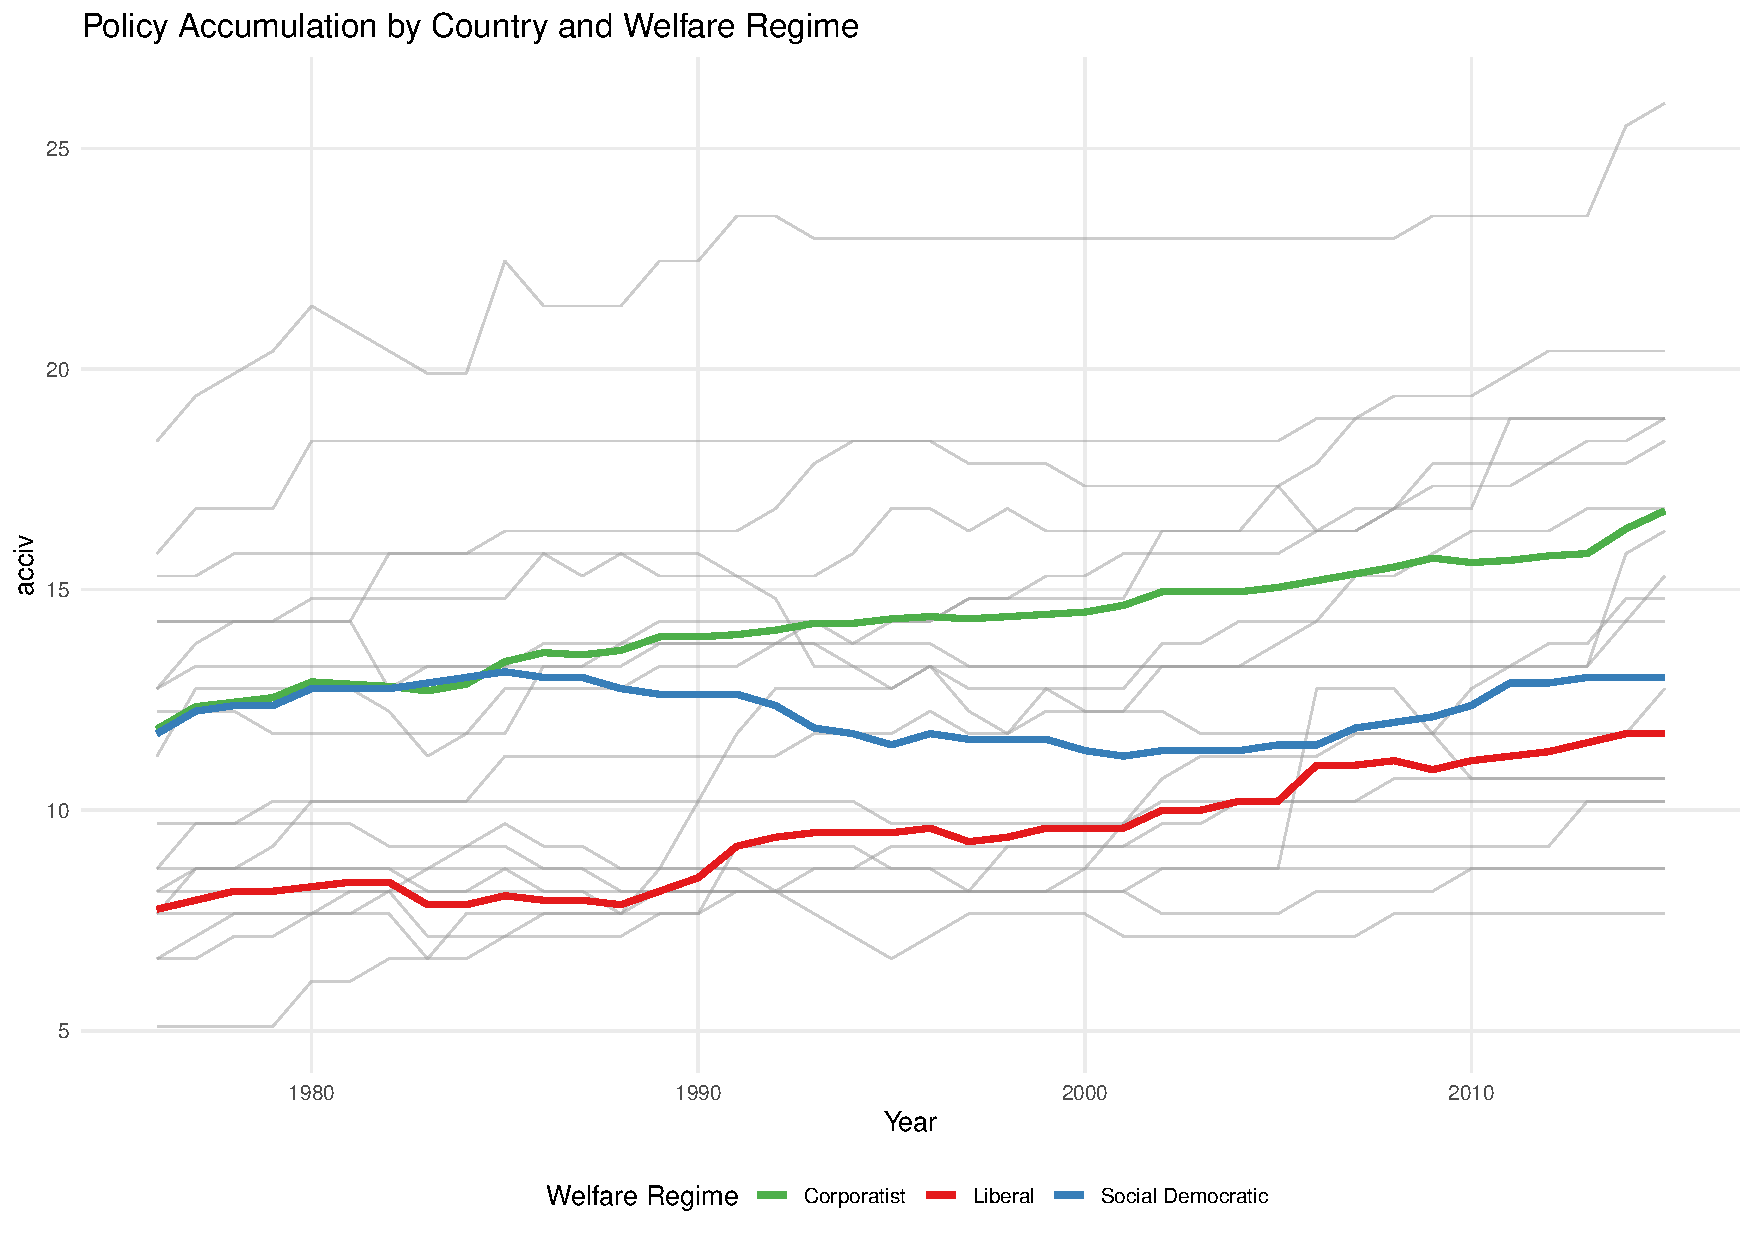
\includegraphics[width=\linewidth]{images/ExamplePlot.pdf}
    \captionof{figure}{An illustrative plot.}
    \label{fig:sidebyside}
\end{minipage}
\hfill
\begin{minipage}{0.5\textwidth}
    \small{
    The plot on the left shows a stylized trend. Because it sits inside a \texttt{minipage} the figure and its caption stay locked together as one block that won't split across a page break.}
\end{minipage}

The number (e.g.\ \verb|0.45\textwidth|) sets how wide each block is relative to the page; the two widths don't need to match --- here the figure takes 0.45 and the text takes 0.5, with \verb|\hfill| filling the remaining space between them so they align to the outer margins.

Note: pairing a minipage with a real \texttt{figure} caption requires the \texttt{caption} package's \verb|\captionof{}| command (since \texttt{figure} environments themselves can't float inside a minipage); if you don't need captions, plain text, tables, or \verb|\includegraphics| alone work fine without extra packages.

\newpage

\subsection*{Extra: TikZ-Pictures}
TikZ is a tool that lets you draw diagrams, flowcharts, causal graphs, and custom illustrations directly in code, rendered as crisp vector graphics that scale perfectly and compile fast (see the earlier tip on PDF vs.\ PNG; TikZ figures are essentially "born" as vector graphics, so you get that benefit automatically). That said, please don't get scared by the code. I've never written TikZ from scratch line by line.

 The practical workflow: describe the diagram you want to an AI assistant (e.g. "a diagram showing four workers connected to two plants, with one plant excluded because it's not linked by any worker moves") and ask for the TikZ code. Compile it as-is first, then tweak only small details afterward --- node positions, colors, spacing --- since these are the parts AI sometimes gets slightly off but are easy to nudge once you see the rendered output.

Below are two real examples from past work, illustrating what's achievable.

\paragraph{Example 1: Illustrating a Connectedness Restriction (AKM Estimation)}
\begin{figure}[H]
\centering
\begin{tikzpicture}[
  >=Stealth,
  font=\small,
  worker/.style={circle, draw=black, very thick, minimum size=8mm, inner sep=0pt},
  plant/.style ={rectangle, draw=black, very thick, minimum size=8mm, inner sep=0pt},
  edge/.style  ={-{Stealth[length=2.2mm,width=2.2mm]}, very thick},
  lcsbox/.style={draw=black, very thick, inner sep=10pt, rounded corners=1pt}
]

\node[worker] (w1) at (0,0.9) {\textbf{1}};
\node[worker] (w2) at (0,0.0) {\textbf{\textcolor{blue}{2}}};

\node[plant]  (A)  at (5.0,0.9) {\textbf{A}};
\node[plant]  (B)  at (5.0,0.0) {\textbf{B}};

\node[lcsbox, fit=(w1)(w2)(A)(B)] (lcs) {};
\node[anchor=south] at ($(lcs.north)!-0.8!(lcs.north east)$) {\textbf{Worker}};
\node[anchor=south] at ($(lcs.north)!0.77!(lcs.north east)$) {\textbf{Plant}};
\node[anchor=north, font=\small] at (lcs.south) {Largest connected set};

\draw[edge] (w1) -- (A);
\draw[edge] (w1) -- (B);
\draw[edge, blue] (w2) -- (B);

\node[worker, draw=black, densely dotted, very thick] (w3) at (0,-1.8) {\textcolor{red}{3}};
\node[plant,  draw=black, densely dotted, very thick] (C)  at (5.0,-1.8) {C};

\draw[edge, red, densely dotted] (w3) -- (C);

\end{tikzpicture}
\caption{Example of the largest connected set used in the AKM estimation.}
\label{fig:example_tikz_1}
\end{figure}

\paragraph{Example 2: Illustrating a Discrete-Time Event-History Setup}
\begin{figure}[H]
\centering
\begin{tikzpicture}[
    font=\small,
    timeline/.style={thick},
    event/.style={circle, fill=black, inner sep=2pt},
    label/.style={font=\footnotesize}
]

\def\tprev{0}
\def\tcurr{3}
\def\tnext{6}

\def\rowA{6}
\def\rowB{4}
\def\rowC{2}
\def\rowD{0}

\def\atriskcolor{gray!20}
\def\realizedcolor{gray!60}

\node[font=\bfseries] at (\tprev, 7.5) {$t-1$};
\node[font=\bfseries] at (\tcurr, 7.5) {$t$};
\node[font=\bfseries] at (\tnext, 7.5) {$t+1$};

\node[anchor=east, font=\footnotesize] at (-0.5, \rowA) {Case 1};
\node[anchor=east, font=\footnotesize] at (-0.5, \rowB) {Case 2};
\node[anchor=east, font=\footnotesize] at (-0.5, \rowC) {Case 3};
\node[anchor=east, font=\footnotesize] at (-0.5, \rowD) {Case 4};

\fill[\atriskcolor] (\tprev-0.5, \rowA-0.4) rectangle (\tnext+0.5, \rowA+0.4);
\draw[timeline] (\tprev, \rowA) -- (\tnext, \rowA);
\node[label, above] at (\tprev, \rowA+0.4) {at risk};
\node[label, above] at (\tcurr, \rowA+0.4) {at risk};
\node[label, above] at (\tnext, \rowA+0.4) {at risk};

\fill[\atriskcolor] (\tprev-0.5, \rowB-0.4) rectangle (\tcurr, \rowB+0.4);
\fill[\realizedcolor] (\tcurr, \rowB-0.4) rectangle (\tnext+0.5, \rowB+0.4);
\draw[timeline] (\tprev, \rowB) -- (\tcurr, \rowB);
\draw[timeline] (\tcurr, \rowB) -- (\tnext, \rowB);
\node[event] at (\tcurr, \rowB) {};
\node[label, above] at (\tprev, \rowB+0.4) {at risk};
\node[label, above] at (\tcurr, \rowB+0.4) {\textbf{event}};
\node[label, above] at (\tnext, \rowB+0.4) {realised};

\fill[\realizedcolor] (\tprev-0.5, \rowC-0.4) rectangle (\tnext+0.5, \rowC+0.4);
\draw[timeline] (\tprev, \rowC) -- (\tnext, \rowC);
\node[label, above] at (\tprev, \rowC+0.4) {realised};
\node[label, above] at (\tcurr, \rowC+0.4) {realised};
\node[label, above] at (\tnext, \rowC+0.4) {realised};

\fill[\realizedcolor] (\tprev-0.5, \rowD-0.4) rectangle (\tcurr, \rowD+0.4);
\fill[\atriskcolor] (\tcurr, \rowD-0.4) rectangle (\tnext+0.5, \rowD+0.4);
\draw[timeline] (\tprev, \rowD) -- (\tcurr, \rowD);
\draw[timeline] (\tcurr, \rowD) -- (\tnext, \rowD);
\node[event, fill=white, draw=black] at (\tcurr, \rowD) {};
\node[label, above] at (\tprev, \rowD+0.4) {realised};
\node[label, above] at (\tcurr, \rowD+0.4) {\textbf{removal}};
\node[label, above] at (\tnext, \rowD+0.4) {at risk};

\draw[dashed, gray] (\tprev, -0.5) -- (\tprev, 7);
\draw[dashed, gray] (\tcurr, -0.5) -- (\tcurr, 7);
\draw[dashed, gray] (\tnext, -0.5) -- (\tnext, 7);

\def\legx{8.0}
\def\legy{5.2}

\node[anchor=west, font=\footnotesize\bfseries] at (\legx, \legy+0.6) {Legend};

\fill[\atriskcolor] (\legx, \legy-0.2) rectangle (\legx+0.4, \legy+0.2);
\node[anchor=west, label] at (\legx+0.55, \legy) {Unrealised (at risk)};

\fill[\realizedcolor] (\legx, \legy-1.0-0.2) rectangle (\legx+0.4, \legy-1.0+0.2);
\node[anchor=west, label] at (\legx+0.55, \legy-1.0) {Realised (not at risk)};

\node[event] at (\legx+0.2, \legy-2.0) {};
\node[anchor=west, label] at (\legx+0.55, \legy-2.0) {Adoption event};

\node[event, fill=white, draw=black] at (\legx+0.2, \legy-3.0) {};
\node[anchor=west, label] at (\legx+0.55, \legy-3.0) {Removal event};

\end{tikzpicture}
\caption{The four possible states of a target-instrument cell across time periods.}
\label{fig:example_tikz_2}
\end{figure}

Both examples above use only the TikZ libraries already loaded in the preamble (\texttt{arrows.meta}, \texttt{positioning}, \texttt{fit}, \texttt{calc}). If you need something more advanced, just ask the AI and mention which libraries you already have loaded.





% ----- BIBLIOGRAPHY -----

\newpage
\bibliography{references}

% ----- APPENDIX or APPENDICES -----
% Contrary to normal sections, the appendix is named A, B, C, etc. Uncomment if needed.

%\newpage
%\appendix
%\input{Sections/Appendix.tex}

\end{document}




